\subsection{CIP-Pool}

Hier nun einige Informationen über die PC-Arbeitsplätze der Mathematik für
Studenten. Es gibt in der ersten Etage des Geomatikums (hinter den Fahrstühlen
rechter Hand) PC Arbeitsplätze für Studenten. 20 Arbeitsplätze mit Windows
Rechnern in den Räumen 142 und 143, und weitere 12 Workstations um unter Unix
zu arbeiten in Raum 144. Dort könnt ihr auf diverse Mathematik-Programme
Internetrecherche und sogar einen kleinen aber persönlichen Speicherort
zugreifen.

\subsubsection{Zugang zu den Rechnern}

Die Poolräume sind unter der Woche zwischen 9:30 und 18:30 geöffnet, in den
vorlesungsfreien Zeiten können diese Öffnungszeiten eingeschränkt sein. In
dieser Zeit ist in der Regel eine Aufsicht als Ansprechpartner vor Ort. Da die
Poolräume nur für Mathematikstudenten gedacht sind (nur Studenten des
Studienbereichs Mathematik und Erziehungswissenschaften) benötigt man eine
Zugangskennung. Diese kann jeder Student im Rechenzentrum (Schlüterstraße 70)
beantragen. Mathematikstudenten (nicht Erziehungswissenschaftler) können dies
auch direkt bei den Poolaufsichten (dauert aber in beiden fällen min. 1 Tag zur
Aktivierung). Beim Anmelden am Rechner muss dann neben Benutzerkennung und
zugehörigen Passwort in der Loginmaske noch angegeben werden welcher
Benutzergruppe ihr angehört. Die Auswahlmöglichkeiten sind \emph{Studi}
(Mathestudent), \emph{Erzwiss} (Lehramtsstudent) und \emph{Mathe}
(Mitarbeiter). Nach dem ersten Anmelden solltet ihr möglichst euer Passwort
ändern. Dies geht nur Online unter www.rrz.uni-hamburg.de $\rightarrow$
Benutzung des RRZ $\rightarrow$ Passwort

\subsubsection{Internet}

Jeder Rechner den ihr in der Uni benutzen könnt hat auch Internetzugang. Wollt
ihr jetzt also Surfen müsst ihr nur noch einen Browser starten. Nutzt bitte den
Firefox der im Novellfenster (startet automatisch beim Login) zu sehen ist.

%\begin{center}
%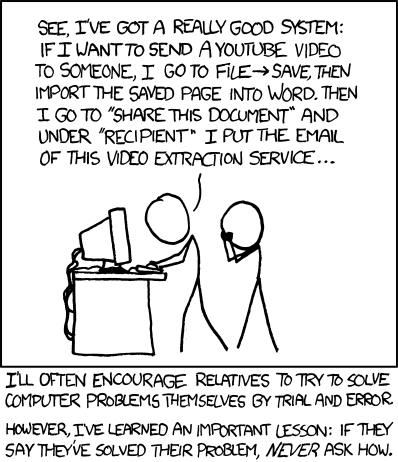
\includegraphics[scale=.8]{comics/763}
%\end{center}

%\begin{center}
%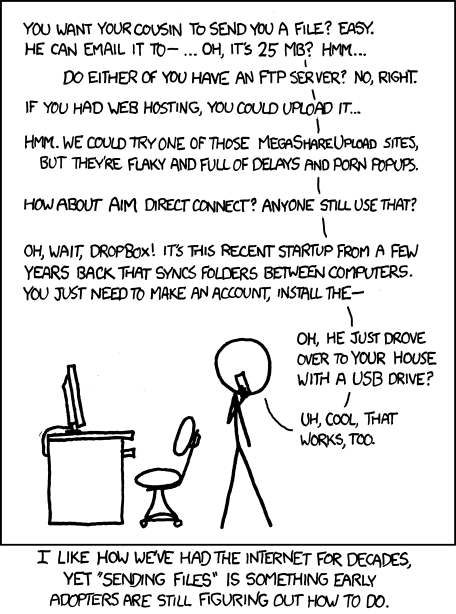
\includegraphics[scale=.85]{comics/949}
%\end{center}

\subsubsection{Speichern und Drucken}

Möchtest du nun Dateien aus dem Internet oder selbst erstellte speichern, hast
du mehrere Möglichkeiten. Alle Windows Rechner haben USB-Schnittstellen für
Speicherchips oder gar USB-Festplatten, ein CD/DVD Laufwerk das auch auf beide
Medien Brennen kann und das gute alte Diskettenlaufwerk. Solltest du nichts
dergleichen zur Hand haben kannst du bis zu 20 MB auf Laufwerk K: speichern.
K: ist ein Netzlaufwerk (also eine Festplatte auf einem Server) auf dem ein
individueller Speicherplatz für dich reserviert ist auf den sonst niemand
zugreifen kann. Als letzte Option bleibt dir noch, Dateien per Mail an dich
selbst zu verschicken.

Alle anderen Speicherorte auf dem Rechner sollten bei deinem Abmelden keine
deiner Dateien mehr enthalten, da andere sonst darauf zugreifen, sie Verändern
oder auch Löschen können was insbesondere die Administratoren auch tun. Was das
Drucken angeht, so gibt es wieder die Möglichkeit für Studenten den Drucker in
Raum 142 (in der Druckerauswahl am Rechner l142) zu nutzen. Mit eurer
Benutzerkennung erhaltet ihr ein monatliches und ausreichendes
Druck-Kontingent.

\subsubsection{E-Mail}

Jeder Student der Uni-Hamburg erhält eine E-Mail-Adresse nach folgendem Muster.

\href{mailto:vorname.nachname@studium.uni-hamburg.de}{vorname.nachname@studium.uni-hamburg.de}

Nutzen und verwalten könnt ihr diese über das Online-Portal des Rechenzentrums
(RRZ) unter \url{http://www.rrz.uni-hamburg.de}. Hier wählt ihr oben rechts den
Link Surfmail und gelangt zur Anmeldemaske, in der ihr mit demselben
Benutzernamen und Passwort auf euer Mailverzeichnis zugreifen könnt, das ihr
auch schon für den Zugang in den Poolräumen genutzt habt.
